\documentclass[a4paper,12pt]{article}   % papír A4, písmo 12 bodu
\usepackage[utf8x]{inputenc}            %kodovaní UTF-8
\usepackage{ucs}                        %kodovani unicode
\usepackage[czech]{babel}               %podpora cestiny
\usepackage[T1]{fontenc}                %pouzij variantu pisma T1 (hacky, carky)
\usepackage[left=2.5cm,right=1.5cm,top=2.5cm,bottom=2.5cm]{geometry} %okraje stranky
\usepackage{amsmath,amsfonts,amssymb}   %podpora matematiky
\usepackage{gensymb,marvosym}           %symboly celsius (\celsius) apod.
%\usepackage{mathptmx}                   %font Times New Roman s~podporou matematiky
\usepackage{times}                      %font Times New Roman (matematika pismem Computer Modern) 
\usepackage{parskip}                    %mezera mezi odstavci
%\usepackage[document]{ragged2e}         %text zarovany vlevo
\usepackage[none]{hyphenat} \sloppy     %slova nedelit a~nepretekat
\usepackage{titlesec}
\setcounter{secnumdepth}{4}
\clubpenalty 10000                      %kontrolovat sirotky
\widowpenalty 10000                     %kontrolovat vdovy
\usepackage{setspace} \onehalfspacing   %podpora pro zmenu radkovani + radkovani 1,5
\usepackage{enumerate}                  %podpora pro zmenu cislovani
\usepackage{fancyhdr}                   %vlastni zahlavi a~zapati
\usepackage{graphicx}                   %podpora grafiky
\graphicspath{{materialy/}}                   %vychozi adresar s~obrazky
\usepackage{caption}                    %popisky
\usepackage{subcaption}                 %podpopisky
\usepackage{siunitx}
\usepackage{MnSymbol,wasysym}
\usepackage[shortlabels]{enumitem}
\usepackage{amsmath}
\usepackage{lastpage}                   %zjištění poslední stránky \pageref{LastPage}
\usepackage{float}                      
\usepackage{url}
\usepackage[unicode]{hyperref}          %klikaci odkazy v~textu
\usepackage{mhchem}
\usepackage{multirow}

\usepackage{halloweenmath}


\titleclass{\subsubsubsection}{straight}[\subsection]
\newcounter{subsubsubsection}[subsubsection]
\renewcommand\thesubsubsubsection{\thesubsubsection.\arabic{subsubsubsection}}
\renewcommand\theparagraph{\thesubsubsubsection.\arabic{paragraph}} % optional; useful if paragraphs are to be numbered


%------------------------ čtvrtá a~pátá úroveň nadpisu ---------------------------

\titleformat{\subsubsubsection}
  {\normalfont\normalsize\bfseries}{\thesubsubsubsection}{1em}{}
\titlespacing*{\subsubsubsection}
{0pt}{3.25ex plus 1ex minus .2ex}{1.5ex plus .2ex}

\makeatletter

\renewcommand\paragraph{\@startsection{paragraph}{5}{\z@}%
  {3.25ex \@plus1ex \@minus.2ex}%
  {-1em}%
  {\normalfont\normalsize\bfseries}}
\renewcommand\subparagraph{\@startsection{subparagraph}{6}{\parindent}%
  {3.25ex \@plus1ex \@minus .2ex}%
  {-1em}%
  {\normalfont\normalsize\bfseries}}
\def\toclevel@subsubsubsection{4}
\def\toclevel@paragraph{5}
\def\toclevel@paragraph{6}
\def\l@subsubsubsection{\@dottedtocline{4}{7em}{4em}}
\def\l@paragraph{\@dottedtocline{5}{10em}{5em}}
\def\l@subparagraph{\@dottedtocline{6}{14em}{6em}}
\makeatother

\setcounter{secnumdepth}{4}
\setcounter{tocdepth}{4}


\setlist[enumerate]{itemsep=0mm}
%_____________________________|___________________________|_____________________________%
%                             |                           |                             %
%-----------------------------| ZDE VYPLNIT UDAJE O PRACI |-----------------------------%
%_____________________________|___________________________|_____________________________%
%                             

\newcommand{\nazev}{MĚŘICÍ USMĚRŇOVAČ}                                                        %
\newcommand{\jmeno}{Jakub Dvořák}                                                     %
\newcommand{\datum}{22.10.2020}                                                              %
%---------------------------------------------------------------------------------------%


%-----------------------------| POUŽITÁ MAKRA |-----------------------------%

%\newcommand{\zkratka}{ve výsledku se mi napíše tenhle text}
%\newcommand{}{}
%\newcommand{}{}
%\newcommand{}{}
\newcommand{\tsub}[1]{$_\textrm{#1}$}
\newcommand{\texp}[1]{$^\textrm{#1}$}
\newcommand{\tohm}{$\Omega$}
\newcommand{\ri}{$R_1$}
\newcommand{\rii}{$R_2$}
\newcommand{\ui}{$U_1$}
\newcommand{\uii}{$U_2$}
\newcommand{\vi}{$V_1$}
\newcommand{\vii}{$V_1$}


%_______________________________________________________________________________________%
%_______________________________________________________________________________________%


%----------------------------------- KONEC PREAMBULE -----------------------------------%






%-------------------------------------- DOKUMENT --------------------------------------%
%______________________________________________________________________________________%
\begin{document} %%%%%%%%%%%%%%%%%%%%%%%%%%%%%%%%%%%%%%%%%%%%%%%%%%%%%%%%%%%%%%%%%%%%%%%

\setcounter{page}{0} %cislo strany
\pagestyle{empty} %stranku necislovat

%prostredi pro grafy a~schemata \begin{graf} \begin{schema}
\newfloat{schema}{htbp}{schema}\floatname{schema}{Schéma}
\newfloat{graf}{htbp}{graf}\floatname{graf}{Graf}

\begin{titlepage}
    \begin{center}
        \vspace*{1cm}
            
        \Huge
        \textbf{\nazev}
            
        \vspace{0.5cm}
        \LARGE
            
        \vspace{1.5cm}
            
        \textbf{\jmeno}
            
        \vfill
            
        \vspace{0.8cm}
            
        \Large
            
        \datum\\
        \vspace*{.5cm}
        
\includegraphics[width=.4\textwidth]{logo-cvut-fee.png}\\
    \end{center}
\end{titlepage}

% --- definice zapati a~cislovani ---
\newpage 
\pagestyle{fancy}                                       %vlastni zahlavi/zapati
\renewcommand{\headrulewidth}{0pt}                      %bez linky v~zahlavi
\renewcommand{\footrulewidth}{.5pt}                    %linka v~zapati - optional
\lhead{}       \chead{} \rhead{\nazev}                        %pole zahlavi (prazdna)
\lfoot{\jmeno} \cfoot{} \rfoot{\thepage}   %pole zapati


%------------------------------------ VLASTNÍ TEXT ------------------------------------%



\section{Úkol měření}
\label{zadani}
\begin{enumerate}
    \item Změřte závislost střední hodnoty výstupního proudu na efektivní hodnotě vstupního napětí polovodičového usměrňovače v~Graetzově zapojení, zatíženého rezistorem \ri = 100~\tohm. Střední hodnotu výstupního proud určete z úbytku napětí na tomto odporu (zapojení dle obr. 1, rozsah stejnosměrného voltmetru \vii~nastavte 200~mV) a~jeho průběh sledujte osciloskopem.
    \item Před polovodičový usměrňovač v~Graetzově zapojení zařaďte odporovou dekádu RD (viz obr. 2) a~experimentálně nastavte hodnotu odporu RD takovou, aby z této kombinace vznikl střídavý číslicový voltmetr s rozsahem 2~V (rozsah stejnosměrného voltmetru \vii~nastavte 200~mV). Změřte závislost stejnosměrného výstupního napětí \uii~na efektivní hodnotě napětí vstupního. Průběh napětí na zatěžovacím rezistoru \rii~sledujte osciloskopem.
    \item Voltmetr se stejným rozsahem jako v~bodě 2 realizujte pomocí operačního zesilovače s usměrňovačem ve zpětné vazbě podle schématu na obr. 3a nebo 3b. Odvoďte příslušný vztah a~vypočtěte hodnotu odporu R\tsub{D} tak, aby efektivní hodnotě vstupního napětí 1~V odpovídala střední hodnota napětí na rezistoru R\tsub{1} U\tsub{R\tsub{1}}~= 100~mV. Experimentálně dostavte hodnotu odporu R\tsub{D}~tak, aby byl tento požadavek skutečně splněn, a~vysvětlete případný rozdíl oproti vypočtené hodnotě.
    \item Opět změřte závislost stejnosměrného výstupního napětí na efektivní hodnotě napětí vstupního. Osciloskopem sledujte nejen průběh proudu, ale i průběh napětí na výstupu OZ. Vysvětlete funkci OZ jako zdroje proudu.
\end{enumerate}
\textit{Poznámka}: Každou závislost změřte v~7 bodech (pro napětí U\tsub{2}~= 5; 10; 25; 50; 100; 150; 200 mV měřené voltmetrem V\tsub{2}). Naměřené průběhy vyneste do společného grafu.

\section{Schéma zapojení}
\label{schema_zapojeni}
\begin{figure}[h!]
    \centering
    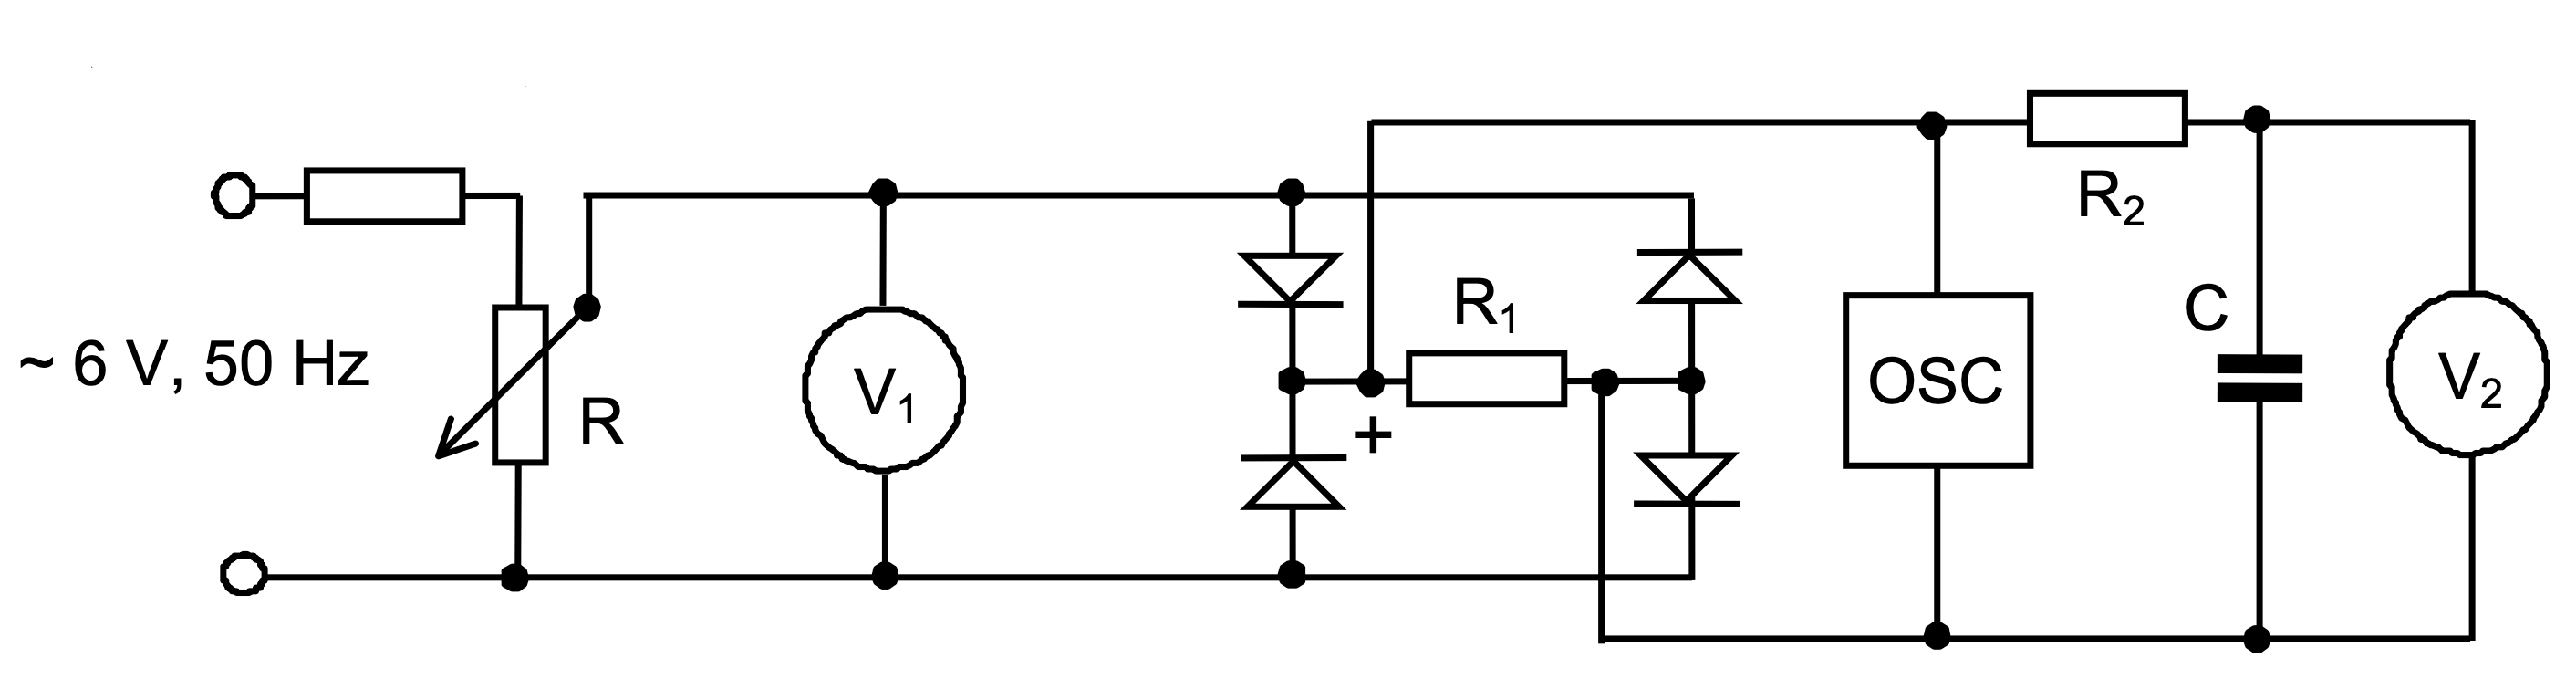
\includegraphics[width=.8\textwidth]{va_char.png}
    \caption{Měření voltampérové charakteristiky usměrňovače zatíženého rezistorem \ri}
    \label{fig:va}
\end{figure}
\begin{figure}[h!]
    \centering
    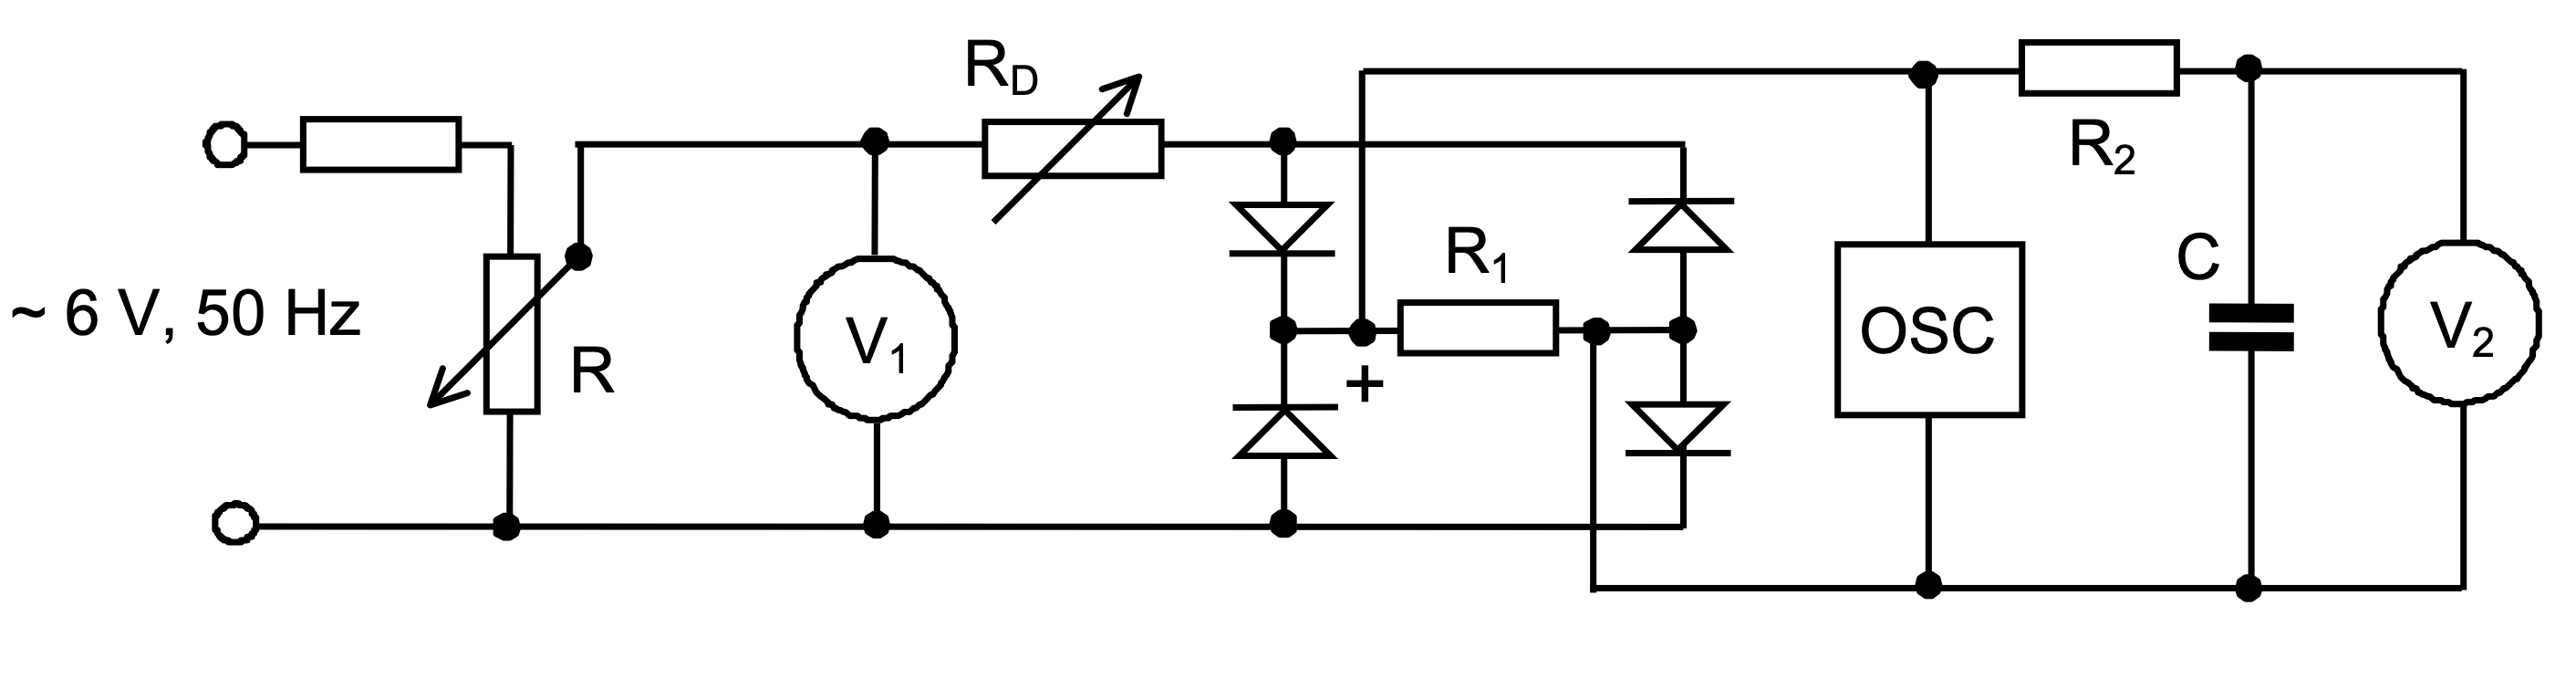
\includegraphics[width=.8\textwidth]{prevod_char.png}
    \caption{Měření převodní charakteristiky sestaveného voltmetru s pasivním usměrňovačem}
    \label{va:prevod}
\end{figure}
\begin{figure}[h!]
    \centering
    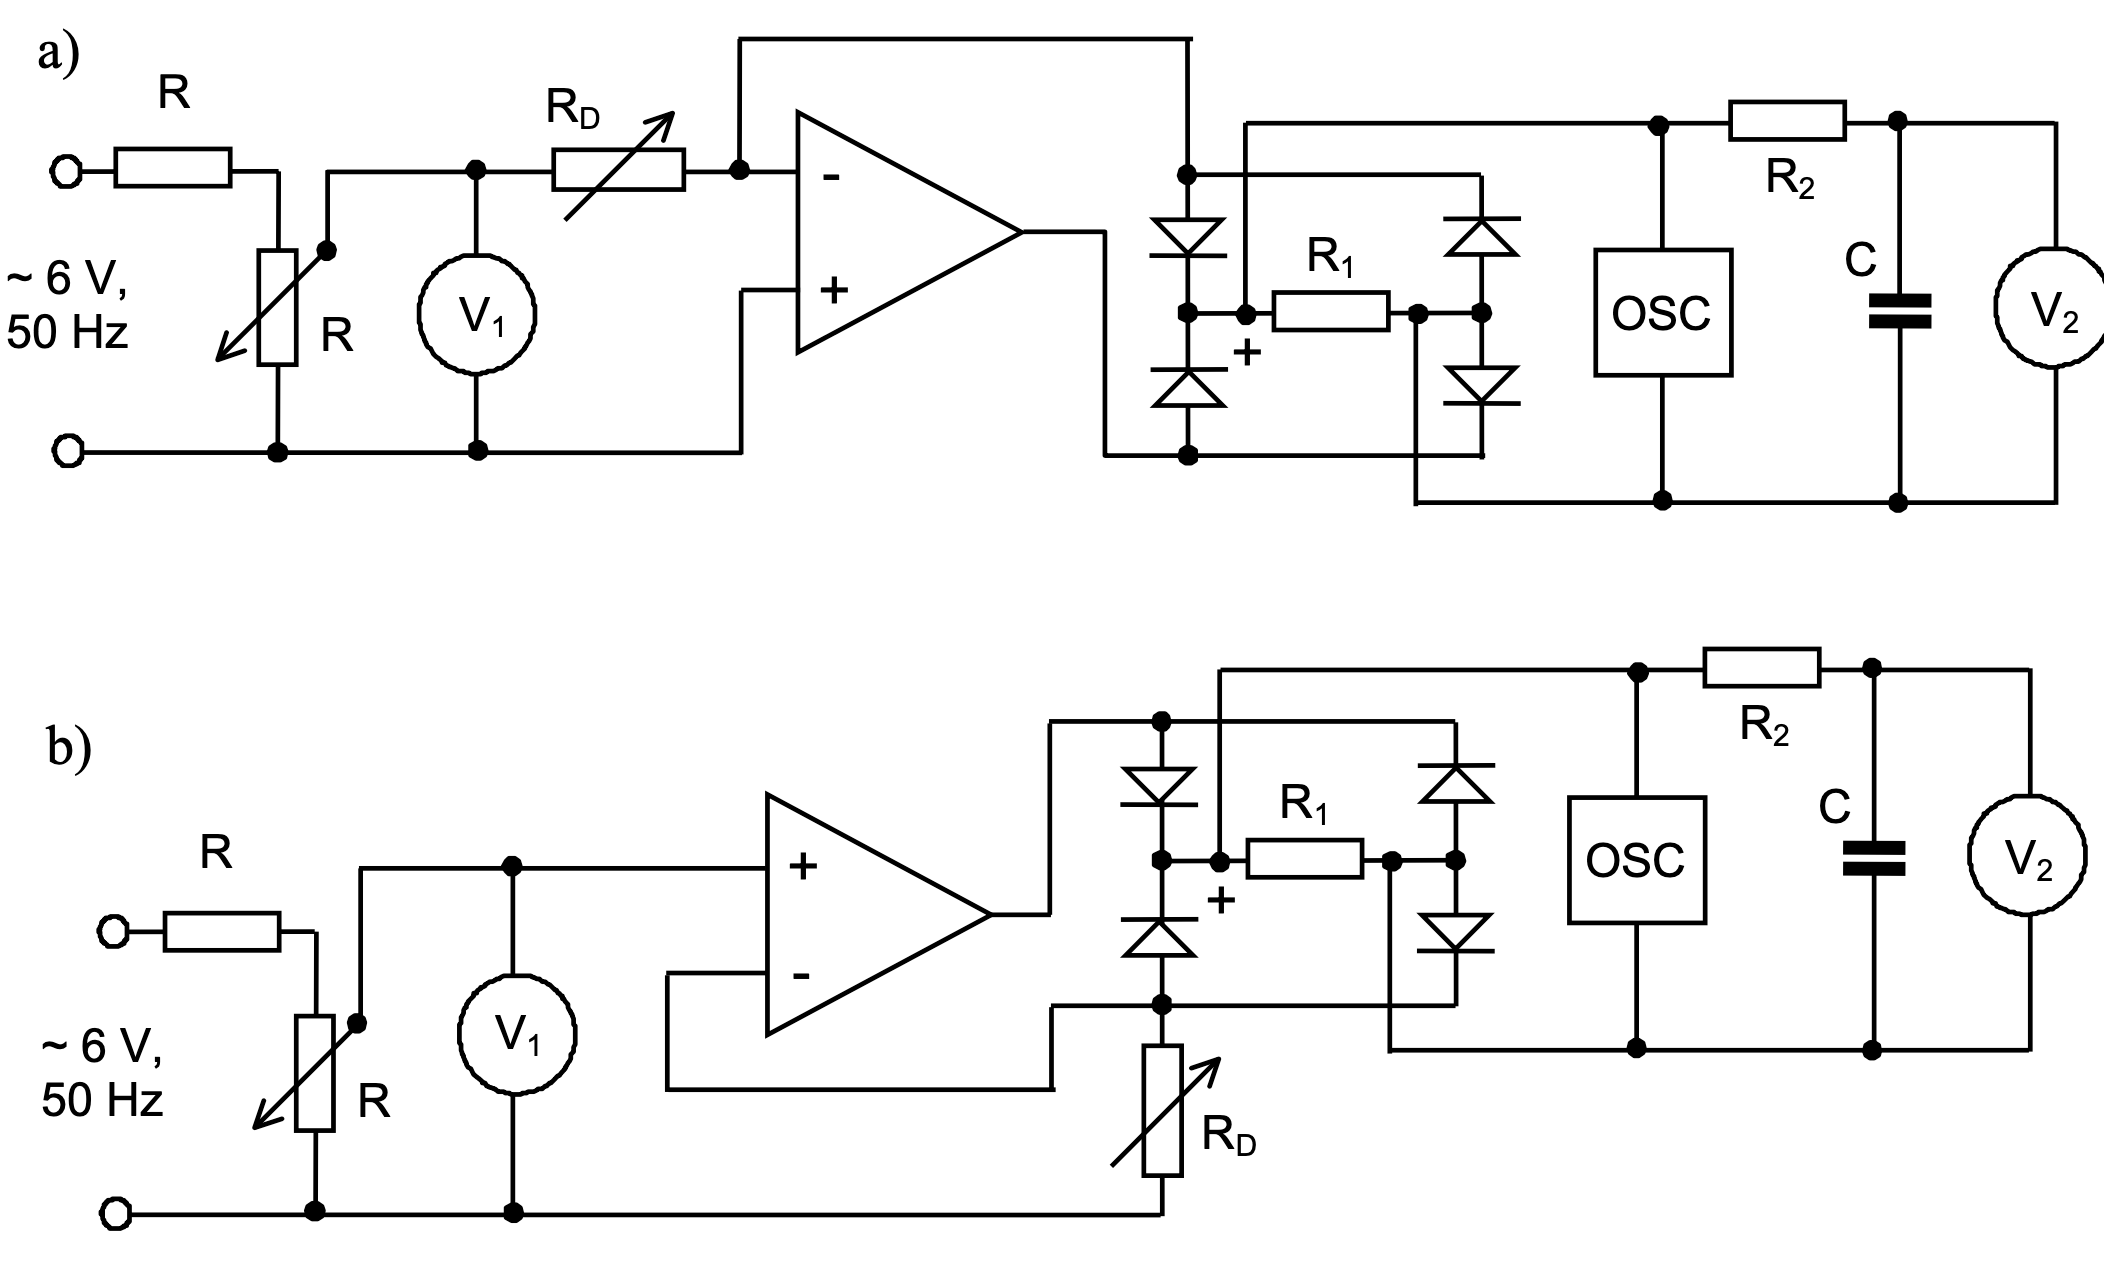
\includegraphics[width=.8\textwidth]{voltmetr.png}
    \caption{Zapojení sestaveného voltmetru s operačním usměrňovačem}
    \label{fig:op}
\end{figure}

\section{Seznam použitých přístrojů}
\begin{itemize}
    \item \vi~Analogový voltmetr střídavý, tř přesnosti 1,5, rozsahy 2,4~V, 6~V
    \item \vii~Digitální multimetr DM-4418, rozsah 200~mV, přesnost (0,1~\% z údaje + 4 digity)\
    \item $Osc$ Osciloskop GoldStar OS-9020G, 20~MHz
    \item $Př_1$ Přípravek s dvoucestným usměrňovačem, zatěžovacím rezistorem \ri~ a~RC filtrem
    \item $Př_2$ Přípravek s operačním zesilovačem
\end{itemize}

\section{Teoretický úvod}
Při měření střídavého napětí je nutno průběh napětí usměrnit. Nejjednodušším způsobem je použití diod v~můstku. Jejich nelineární VA charakteristika jim ale nedovoluje přesné měření v~oblasti, kdy se napětí na diodách pohybuje pod, nebo v~oblasti dopředného napětí. Tato vlastnost jde kompenzovat předřadným odporem, čímž zlinearizujeme větší část u počátku, ale stále se jedná o nelineární charakteristiku. Měřící přístroje využívající diodového můstku často nemají při začátku rozsahu stupnici, jelikož nelze provést přesné měření. Řešením je použití můstku s operačním zesilovačem ve zpětné vazbě viz obr. \ref{fig:op}.

Odpor odporové dekády $R_D$ vypočítáme následovně: 
\begin{equation*}
    \begin{split}
        \frac{U_2}{R_1} &= \frac{U_{1_S}}{R_D} \\
        U_{ef} &= U_{str}/1,11\\
        R_D &= \frac{U_{1_S}\cdot R_1}{U_2\cdot 1,11}\\
    \end{split}
\end{equation*}
\begin{equation*}
    R_D= \frac{U_{1_S}\cdot R_1}{U_2\cdot 1,11} = \frac{1\cdot 100}{1,11\cdot 0,1} = 900,9 \Omega
\end{equation*}


\section{Naměřené hodnoty}
Naměřené hodnoty jsou v~tabulkách níže. Výstupní proud byl počítán jako $I_2=U_2/R_1$, kde $R_1$~=~100~\tohm.

\begin{table}[h!]
    \centering
    \begin{tabular}{|c|c|c|}
        \hline
        $U_{vstup}$ Analogový voltmetr [V] &$U_{2}$ DM-4418 [mV] &Výstupní proud [mA] \\\hline\hline
        1,18    &195,5  &1,955  \\\hline
        1,09    &149,45 &1,4945 \\\hline
        0,99    &103,25 &1,0325 \\\hline
        0,88    &50,99  &0,5099 \\\hline
        0,78    &24,52  &0,2452 \\\hline
        0,72    &9,81   &0,0981 \\\hline
        0,66    &5,37   &0,0537 \\\hline
        0       &0,13   &0,0013 \\\hline
    \end{tabular}
    \caption{První měření}
\end{table}

\begin{table}[h!]
    \centering
    \begin{tabular}{|c|c|c|}
        \hline
        $U_{vstup}$ Analogový voltmetr [V] &$U_{2}$ DM-4418 [mV] &Výstupní proud [mA] \\\hline\hline
        2,02&195,62&1,9562\\\hline
        1,74&151,38&1,5138\\\hline
        1,45&101,05&1,0105\\\hline
        1,13&50,67&0,5067\\\hline
        0,95&24,45&0,2445\\\hline
        0,78&10,28&0,1028\\\hline
        0,7&5,32&0,0532\\\hline
        0&0,13&0,0013\\\hline
    \end{tabular}
    \caption{Druhé měření}
\end{table}

\begin{table}[h!]
    \centering
    \begin{tabular}{|c|c|c|}
        \hline
        $U_{vstup}$ Analogový voltmetr [V] &$U_{2}$ DM-4418 [mV] &Výstupní proud [mA] \\\hline\hline
        1&99,99&0,9999\\\hline
        0,72&71,62&0,7162\\\hline
        0,52&49,66&0,4966\\\hline
        0,27&26,78&0,2678\\\hline
        0,05&5,79&0,0579\\\hline
        0&0,17&0,0017\\\hline
    \end{tabular}
    \caption{Třetí měření}
\end{table}


\section{Zpracování naměřených hodnot}

\begin{graf}[h!]
    \centering
    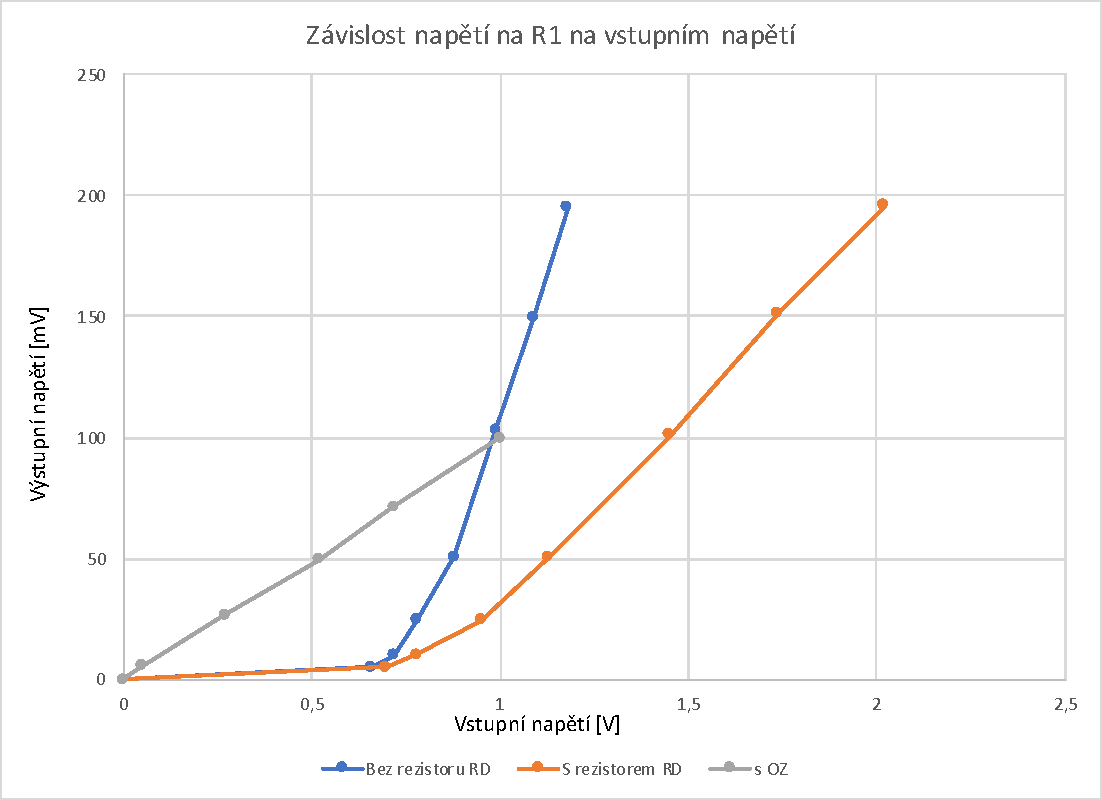
\includegraphics[width=.7\textwidth]{napeti.pdf}
    \caption{Závislost napětí na R1 v~závislosti na vstupním napětí}
\end{graf}

\begin{graf}[h!]
    \centering
    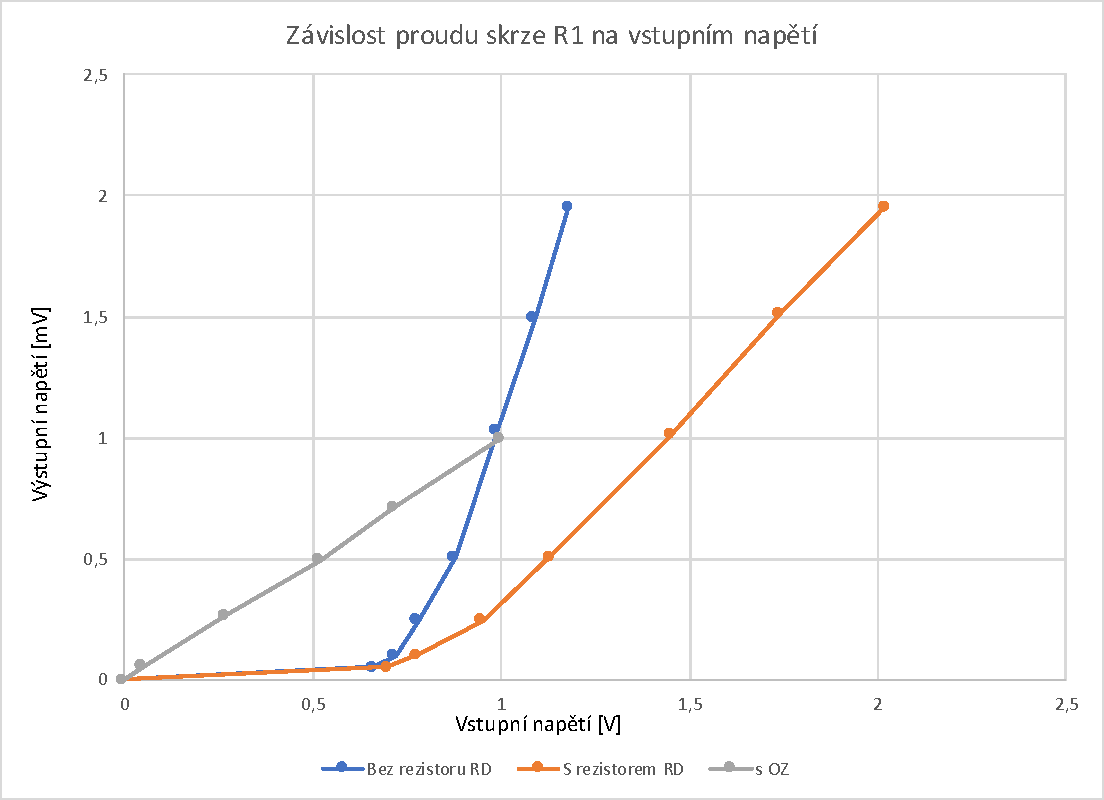
\includegraphics[width=.7\textwidth]{proud.pdf}
    \caption{Závislost proudu skrz R1 v~závislosti na vstupním napětí}
\end{graf}

\section{Závěrečné vyhodnocení}
Zjistili jsme, že diody se nechovají lineárně, pokud jde o malá napětí. To je způsobeno dopředným napětím, při kterém ze diody začínají výrazněji otevírat (dopředné napětí je dáno typem diody). Z grafů je vidět, že dopředné napětí pro naše diody se pohybuje kolem 0,7~V, což je typická hodnota. Také jsme ověřili, že při použití zpětné vazby pomocí operačního zesilovače můžeme dosáhnout velice lineární VA charakteristiky.


%--- LITERATURA a~ZDROJE (povinne) ---
\clearpage
\renewcommand{\refname}{Seznam použité literatury a~zdrojů informací} 
%\section*{Seznam použité literatury a~zdrojů informací}
\phantomsection %pridej odkaz do PDF zalozek
\addcontentsline{toc}{section}{Seznam použité literatury a~zdrojů informací}

\begin{thebibliography}{99}

%----------------------------------------------------
\subsection*{Seznam použitých internetových zdrojů}
    \bibitem{navod} Návod k laboratorní úloze
    
\end{thebibliography}

\end{document}